\documentclass[12pt]{beamer}

\usetheme{Air}
\usepackage{thumbpdf}
\usepackage{wasysym}
\usepackage{ucs}
\usepackage[utf8]{inputenc}
\usepackage{pgf,pgfarrows,pgfnodes,pgfautomata,pgfheaps,pgfshade}
\usepackage{verbatim}
\usepackage{listings}
\usenavigationsymbolstemplate{}

\pdfinfo
{
  /Title       (ANDROID)
  /Creator     (LATEX)
  /Author      (RAFAEL FERNANDEZ LOPEZ)
}

\lstset{ %
    basicstyle=\scriptsize,
    frame=single,
    tabsize=2,
    breaklines=true,
    breakatwhitespace=false
}

\title{Android}
\subtitle{AISO}
\author{Rafael Fernández López}
\date{Abril, 2011}

\begin{document}

\begin{frame}{AISO - Android}
  \framesubtitle{ereslibre@kde.org}
  \titlepage
\end{frame}

\section*{}
\begin{frame}
  \frametitle{AISO - Android}
  \tableofcontents[section=1,hidesubsections]
\end{frame}

\AtBeginSection[]
{
  \frame<handout:0>
  {
    \frametitle{AISO - Android}
    \tableofcontents[currentsection,hideallsubsections]
  }
}

\section{¿Qué es Android?}

\begin{frame}{¿Qué es Android?}
    \framesubtitle{}
    \begin{itemize}
        \item Sistema Operativo
        \item Middleware
        \item Aplicaciones y Servicios
        \item Desde arriba
    \end{itemize}
\end{frame}

\begin{frame}{¿Qué es Android?}
    \framesubtitle{Sistema Operativo}
    \begin{itemize}
        \item Linux Kernel
        \begin{itemize}
            \item Versión
            \begin{itemize}
                \item 2.6.X (2.6.36 actualmente)
            \end{itemize}
            \item Sistema de Ficheros
            \begin{itemize}
                \item YAFFS (Yet Another Flash File System)
            \end{itemize}
            \item Planificador
            \begin{itemize}
                \item CFS (Completely Fair Scheduler)
            \end{itemize}
        \end{itemize}
        \bigskip
        \item Arquitectura
        \begin{itemize}
            \item ARM
        \end{itemize}
    \end{itemize}
\end{frame}

\begin{frame}{¿Qué es Android?}
    \framesubtitle{Middleware}
    \begin{itemize}
        \item Core (Apache Harmony)
        \item IPC Propio (Inter-Process Communication)
        \item Librería C de acceso al sistema
        \item Librerías multimedia
        \item Manejador de superficies
        \item LibWebCore
        \item SGL
        \item Librerías 3D
        \item FreeType
        \item SQLite
    \end{itemize}
\end{frame}

\begin{frame}{¿Qué es Android?}
    \framesubtitle{Aplicaciones y Servicios}
    \begin{itemize}
        \item De interés general
        \begin{itemize}
            \item Home
            \item Agenda
            \item Telefonía
            \item Mensajería
            \item Navegador
            \item Market
            \item Reproductor Multimedia
        \end{itemize}
        \item Google
        \begin{itemize}
            \item Mensajería instantánea (Google Talk)
            \item Google Maps
            \item Google Places
            \item Google Calendar
            \item Navigator (Google Navigator)
            \item Galería (Google Picasa)
        \end{itemize}
    \end{itemize}
\end{frame}

\begin{frame}{¿Qué es Android?}
    \framesubtitle{Desde arriba}
    \center
    \begin{figure}
        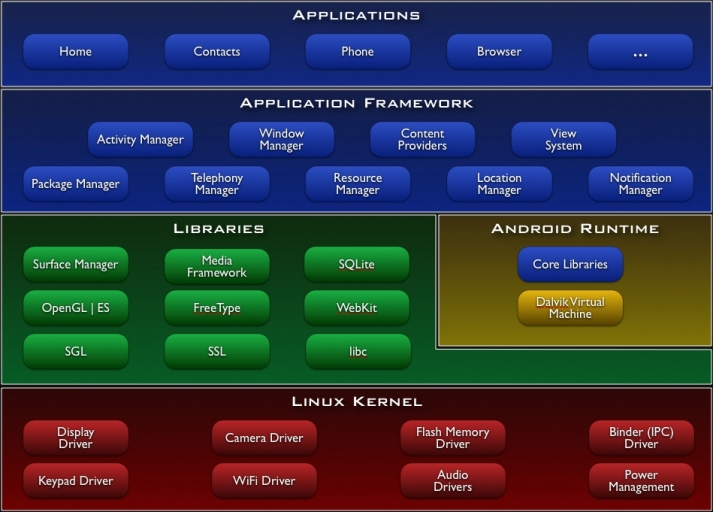
\includegraphics[width=10cm]{android-architecture.jpg}
    \end{figure}
\end{frame}

\section{Historia}

\begin{frame}{Historia}
    \framesubtitle{}
    \begin{itemize}
        \item Android Inc. fundado en 2003
        \item Android Inc. comprado por Google en 2005
        \item Open Handset Alliance revela Android en 2007
        \item Versiones
        \begin{itemize}
            \item 1.5 (Cupcake) - 2.6.27
            \item 1.6 (Donut) - 2.6.29
            \item 2.0 (Eclair) - 2.6.29
            \item 2.2 (Froyo) - 2.6.32
            \item 2.3 (Gingerbread) - 2.6.33
            \item 3.0 (Honeycomb) - 2.6.35
            \item 3.? (Ice Cream Sandwich) - 2.6.??
        \end{itemize}
    \end{itemize}
\end{frame}

\section{Diseño}

\begin{frame}{Dalvik}
    \framesubtitle{}
    \begin{itemize}
        \item Máquina virtual de Google
        \item Bytecode propio
        \item Código fuente en Java $rightarrow$ javac $rightarrow$ .class $rightarrow$ dx $rightarrow$ .dex
        \item Basada en registros $\rightarrow$ no es una máquina basada en pila
        \item Una máquina virtual en ejecución por aplicación
    \end{itemize}
\end{frame}

\begin{frame}{Dalvik}
    \framesubtitle{Consumo de memoria}
    \begin{itemize}
        \item Compartición de regiones
        \begin{itemize}
            \item Sólo lectura
            \item Escritura
            \begin{itemize}
                \item Copy-on-write
            \end{itemize}
        \end{itemize}
    \end{itemize}
\end{frame}

\begin{frame}{Dalvik}
    \framesubtitle{Seguridad}
    \begin{itemize}
        \item Aplicaciones enjauladas
    \end{itemize}
\end{frame}

\section{Peculiaridades}

\begin{frame}{Visión de los procesos}
    \begin{itemize}
        \item Los procesos son contenedores
        \item No existe la relación Aplicación $\leftrightarrow$ Proceso
        \item Multitasking en background
        \begin{itemize}
            \item Broadcast receivers
            \item Servicios
        \end{itemize}
        \item kill -9 cuando se necesita memoria
        \begin{itemize}
            \item Guarda estado de aplicación
            \item Restaura en caso de ser necesario
        \end{itemize}
    \end{itemize}
\end{frame}

\begin{frame}{Actividades}
    \center
    \begin{figure}
        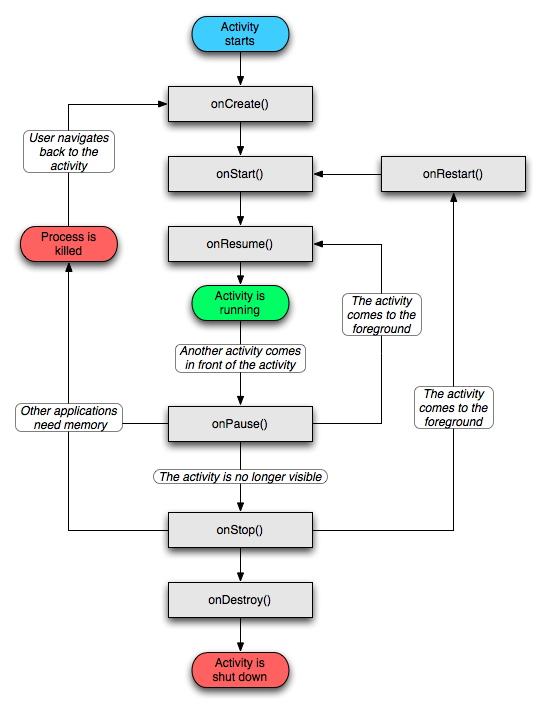
\includegraphics[width=5.8cm]{activity_lifecycle.png}
    \end{figure}
\end{frame}

\begin{frame}[fragile]{Diferencias con el Kernel}
    \framesubtitle{2.6.36}
    \begin{lstlisting}
364 files changed, 93369 insertions(+), 383 deletions(-)
    \end{lstlisting}
    \begin{itemize}
        \item Kernel
        \begin{itemize}
            \item Auto terminación de procesos
            \item Wakelocks
            \item Suspendido rápido
            \item ashmem
            \item Panic timeout
            \item Cambios en cgroup/cset
            \item Cambios en futexes
            \item sysctl para sistemas sin swap
        \end{itemize}
        \item Drivers
    \end{itemize}
\end{frame}

\begin{frame}[fragile]{Diferencias con el Kernel}
    \framesubtitle{2.6.36}
    \begin{itemize}
        \item Red
        \begin{itemize}
            \item PPP en L2TP controlador de acceso
            \item PPP en PPTP servidor de red
            \item Ficheros sysfs para control de red
        \end{itemize}
        \item Sistema de Ficheros
        \begin{itemize}
            \item YAFFS2
            \item ioctl para ID de Volúmenes FAT
            \item Cambios en inotify
            \item uevents por partición
            \item Sistema de ficheros procfs especial
        \end{itemize}
    \end{itemize}
\end{frame}

\frame{
  \frametitle{AISO - Android}
  \vspace{1.5cm}
  {\huge \alert{\textbf{Gracias.}} ¿Preguntas?}

  \vspace{1cm}
  \begin{center}
    \large \textbf{http://www.android.com/}
  \end{center}


  \vspace{1cm}
  \begin{flushright}
    Rafael Fernández López

    \structure{\footnotesize{ereslibre@kde.org}}
  \end{flushright}
}

\end{document}
